\documentclass[cjk,slidestop,compress,mathserif,blue]{beamer}
%dvipdfm选项是关键,否则编译统统通不过
%beamer的颜色选项定义的是导航条和标题的颜色(即关键词structure的颜色)

%%%%%%%%%%%%%%%%仅限于XeTeX可使用的宏包%%%%%%%%%%%%%%%%%%%%%%%%%%%%
\usepackage{fontspec,xunicode,xltxtra,beamerthemesplit}
%\usepackage{beamerthemesplit}
\usepackage{handoutWithNotes}		%(讲义)在打印PPT的时候会留出给每一页做注释的部分
\usepackage{xeCJK}
\setCJKmainfont[BoldFont=黑体, ItalicFont=楷体, BoldItalicFont=仿宋]{黑体}
%\setsansfont[Mapping=tex-text]{Adobe 黑体 Std}
%如果装了Adobe Acrobat,可在font.conf中配置Adobe字体的路径以使用其中文字体
%也可直接使用系统中的中文字体如SimSun,SimHei,微软雅黑 等
%原来beamer用的字体是sans family;注意Mapping的大小写,不能写错

\usepackage{listings} 
\lstset{language=Matlab}%代码语言使用的是matlab 
\lstset{breaklines}%自动将长的代码行换行排版 
\lstset{extendedchars=false}%解决代码跨页时,章节标\dots

%%%%%%%%   确定标题和导航条结构的框架     %%%%%%%%%%%%
\usepackage{beamerthemeshadow}                       %
%\usepackage{beamerthemeclassic}%导航条色与背景色一致%
%%%%%%%%%%%%%%%%%%%%%%%%%%%%%%%%%%%%%%%%%%%%%%%%%%%%%%
\setbeamerfont{roman title}{size={}}
%\usepackage{CJK} % CJK 中文支持                                  %
\usepackage{amsmath,amsthm,amsfonts,amssymb,bm}
\usepackage{bbding}
\usepackage{mathrsfs}
\usepackage{xcolor}                                        %使用默认允许使用颜色
\usepackage{hyperref} 
\usepackage{graphicx}
\usepackage{subfigure}           %图片跨页
\usepackage{animate}		 %插入动画
\usepackage{tikz}		 %绘图工具
\usepackage{caption}
\captionsetup{font=footnotesize}

%\usepackage[version=3]{mhchem}		%化学公式
\usepackage{chemformula}
\usepackage{chemfig}		%化学公式

\usepackage{multirow}
\usepackage{makecell}		%允许单元格内换行

\usepackage[dvipdfmx]{movie15_dvipdfmx} %插入视频
%\usepackage{handoutWithNotes}		%(讲义)在打印PPT的时候会留出给每一页做注释的部分
%\pgfpagesuselayout{1 on 1 with notes landscape}[a4paper,border shrink=5mm]

%%%%%%%%%%%%%%%%%%%%%%BIBTEX 引用参考文献%%%%%%%%%%%%%%%%%%%%%%%%%%%%%%%%%%%%%%%%%%%%%%%%
%\usepackage{filecontents}
%\begin{filecontents*}{main.bib}
%@techreport{2012FracfocusChemical,
%  author = {FracFocus,},
%  howpublished = {\url{http://fracfocus.org/water-protection/drilling-usage}},
%  institution = {The Ground Water Protection Council and Interstate Oil and Gas
%  Compact Commission},
%  month = {feb},
%  title = {{Chemical Use In Hydraulic Fracturing}},
%  year = {2012}
%}
%\end{filecontents*}
%\usepackage[backend=bibtex,sorting=none]{biblatex}
%%\usepackage[backend=biber,style=authoryear]{biblatex}
%\addbibresource{main.bib} %BibTeX数据文件及位置

%\usepackage[numbers,sort&compress]{natbib} %紧密排列             %
\usepackage[sectionbib]{chapterbib}        %每章节单独参考文献   %
\usepackage{hypernat}                                                                         %
\setbeamertemplate{bibliography item}[text] %参考文献前标注[]
%\usepackage[dvipdfm,bookmarksopen=true,pdfstartview=FitH,CJKbookmarks]{hyperref}		%
\hypersetup{bookmarksnumbered,colorlinks,linkcolor=brown,citecolor=blue,urlcolor=red}         %
%参考文献含有超链接引用时需要下列宏包,注意与natbib有冲突        %
%\usepackage[dvipdfm]{hyperref}                                  %
%\usepackage{hypernat}                                           %
\newcommand{\upcite}[1]{\hspace{0ex}\textsuperscript{\cite{#1}}} %

%\usepackage{marvosym} %插入各种符号

%\useoutertheme{smoothbars}
\useinnertheme[shadow=true]{rounded}
\usetheme{Berkeley}                                          %主题式样
%\usetheme{Luebeck}

\usecolortheme{lily}                                        %颜色主题式样

\usefonttheme{professionalfonts}                           %字体主题样式宏包

%\beamertemplatetransparentcoveredhigh                      %使所有被隐藏的文本高度透明
\beamertemplatetransparentcovereddynamicmedium             %使所有被隐藏的文本完全透明,动态,动态的范围很小
\mode<presentation>
%\beamersetaveragebackground{gray}                          %设置背景颜色(单一色) 
\beamertemplateshadingbackground{green!10}{red!5}         %设置背景颜色(渐变色)

%i放置单位logo
%\logo{
\includegraphics[width=1.6cm,height=0.35cm]{Figures/BCC_logo-1.png}}	%简单设置logo

%\pgfdeclareimage[width=3.5cm]{logoname}{Figures/BCC_logo-1.png}		%logo置于左侧微调
%\logo{\pgfuseimage{logoname}{\vspace{0.2cm}\hspace*{-2.0cm}}}

%在指定位置精确放置logo
\usepackage{tikz}
\usepackage{beamerfoils}
\usepackage{pgf}
\logo{\pgfputat{\pgfxy(11.68,0.15)}{
\includegraphics[height=1.01cm,viewport=0 0 140 120,clip]{Figures/BCC_logo-1.png}}\pgfputat{\pgfxy(10.502,-0.218)}{
\includegraphics[height=0.369cm,viewport=140 0 540 120,clip]{Figures/BCC_logo-1.png}}}
%\logo{\pgfputat{\pgfxy(11.68,0.15)}{
\includegraphics[height=0.95cm,viewport=0 0 510 360,clip]{Figures/Logo_Gainstrong.png}}\pgfputat{\pgfxy(10.333,-0.195)}{
\includegraphics[height=0.35cm,viewport=530 70 1100 218,clip]{Figures/Logo_Gainstrong.png}}}
%\logo{\pgfputat{\pgfxy(10.28,0.00)}{
\includegraphics[height=0.95cm,viewport=0 0 1100 360,clip]{Figures/Logo_Gainstrong.png}}}
%\logo{\pgfputat{\pgfxy(11.68,0.15)}{
\includegraphics[height=0.95cm,viewport=0 0 510 360,clip]{Figures/Logo_Gainstrong.png}}\pgfputat{\pgfxy(10.333,-0.195)}{
\includegraphics[height=0.35cm,viewport=530 70 1100 218,clip]{Figures/Logo_Gainstrong.png}}}
%\MyLogo{
%	\pgfputat{\pgfxy(-50,-50)}{\pgfbox[right,base]{
\includegraphics[height=1cm]{Figures/BCC_logo-1.png}}}

%logo作为背景放置
%\setbeamertemplate{background}{
%	\pgfputat{\pgfxy(6.5,-0.5)}{\pgfbox[left,top]{\pgfimage[height=1.1cm]{Figures/BCC_logo-1.png}}}}

%\logo{}									%不显示logo

\begin{document}
%\begin{CJK*}{GBK}{song}
%\begin{CJK*}{GBK}{kai}
%beamer下不能用\songyi、\zihao等命令!
%\graphicspath{Figures/}

%\renewcommand{\figurename}{\tiny\CJKfamily{hei} 图.}
\renewcommand{\figurename}{\tiny{\bf Fig}.}
%\renewcommand{\tablename}{\tiny\CJKfamily{hei} 表.}
\renewcommand{\tablename}{\tiny{\bf Tab}.}
%\renewcommand{\tablename}{\tiny\CJKfamily{hei} 表.}
%\renewcommand{\thesubfigure}{\roman{subfigure}}  %\makeatletter 子图标记罗马字母
\renewcommand{\thesubfigure}{\tiny(\alph{subfigure})}  %\makeatletter 子图标记英文字母
%\renewcommand{\thesubfigure}{}  \makeatletter %子图无标记

%%%%%%%%%%%%%%%%%%%%%%%%%%%%%%% Latex 的 tikz 绘图 %%%%%%%%%%%%%%%%%%%%%%%%%%%%%%%%%%%%%%%%%%%
%\begin{tikzpicture}
%    % 引入图片
%    \node[anchor=south west,inner sep=0] (image) at (0,0) {\includegraphics[width=0.9\textwidth]{Mycena_interrupta.jpg}};
%
%    \begin{scope}[x={(image.south east)},y={(image.north west)}]
%        % 建立相对坐标系
%        \draw[help lines,xstep=.1,ystep=.1] (0,0) grid (1,1);
%        \foreach \x in {0,1,...,9} { \node [anchor=north] at (\x/10,0) {0.\x}; }
%        \foreach \y in {0,1,...,9} { \node [anchor=east] at (0,\y/10) {0.\y}; }
%        % 作图命令
%        \draw[red, ultra thick, rounded corners] (0.62,0.65) rectangle (0.78,0.75);
%    \end{scope}
%\end{tikzpicture}
%%%%%%%%%%%%%%%%%%%%%%%%%%%%%%%%%%%%%%%%%%%%%%%%%%%%%%%%%%%%%%%%%%%%%%%%%%%%%%%%%%%%%%%%%%%%%%

%-------------------------------PPT Title-------------------------------------
\title{软件\rm{MagGene}简介}
%-----------------------------------------------------------------------------

%----------------------------Author & Date------------------------------------
\author[\textrm{Jun\_Jiang}]{姜\;\;骏\inst{}} %[]{} (optional, use only with lots of authors)
% - Give the names in the same order as the appear in the paper.
% - Use the \inst{?} command only if the authors have different
%   affiliation.
\institute[BCC]{\inst{}%
 \vskip -20pt 北京市计算中心}
\date[\today] % (optional, should be abbreviation of conference name)
{	%{\fontsize{6.2pt}{4.2pt}\selectfont{\textcolor{blue}{E-mail:~}\url{jiangjun@bcc.ac.cn}}}
\vskip 45 pt {\fontsize{8.2pt}{6.2pt}\selectfont{%北京理工大学%报告地点
	\vskip 5 pt \textrm{2020.11.28}}}
}

% - Either use conference name or its abbreviation
% - Not really information to the audience, more for people (including
%   yourself) who are reading the slides online

\subject{}
% This is only inserted into the PDF information catalog. Can be left
% out.
\frame
{
%	\frametitle{\fontsize{9.5pt}{5.2pt}\selectfont{\textcolor{orange}{“高通量并发式材料计算算法与软件”年度检查}}}
\titlepage
}
%-----------------------------------------------------------------------------

%------------------------------------------------------------------------------列出全文 outline ---------------------------------------------------------------------------------
\section*{}
\frame[allowframebreaks]
{
  \frametitle{Outline}
%  \frametitle{\textcolor{mycolor}{\secname}}
  \tableofcontents%[current,currentsection,currentsubsection]
}
%在每个section之前列出全部Outline
%类似的在每个subsection之前列出全部Outline是\AtBeginSubsection[]
\AtBeginSection[]
{
  \frame<handout:0>%[allowframebreaks]
  {
    \frametitle{Outline}
%全部Outline中,本部分加亮
    \tableofcontents[current,currentsection]
  }
}

%------------------------------------------------------------------------------PPT main Body------------------------------------------------------------------------------------
\small
%\section{引言}
\frame
{
	\frametitle{科学研究的范式变更}
\begin{figure}[h!]
\vspace*{-0.18in}
\centering
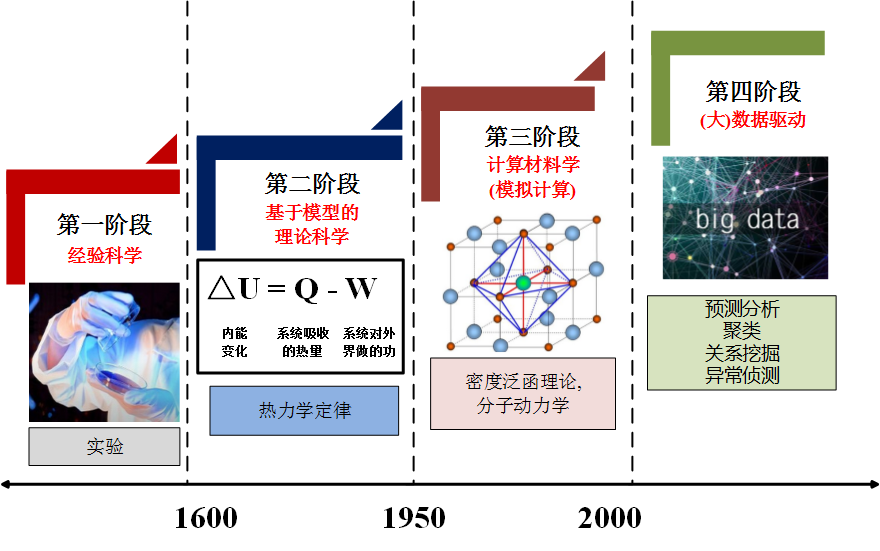
\includegraphics[width=4.05in]{Figures/Four_Model.png}
%\caption{\tiny \textrm{Pseudopotential for metallic sodium, based on the empty core model and screened by the Thomas-Fermi dielectric function.}}%(与文献\cite{EPJB33-47_2003}图1对比)
\label{Four_Model}
\end{figure}
}

\frame
{
	\frametitle{材料模拟的基本思想和方法}
\begin{figure}[h!]
\vspace*{-0.20in}
\centering
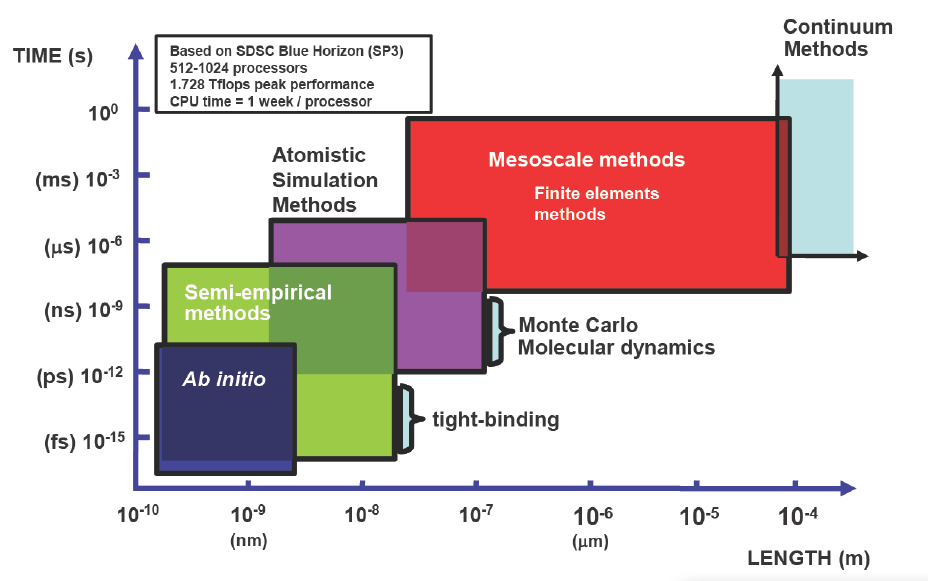
\includegraphics[height=2.20in,width=3.45in]{Figures/Multi-Scale-6.png}
\vskip 0.05pt
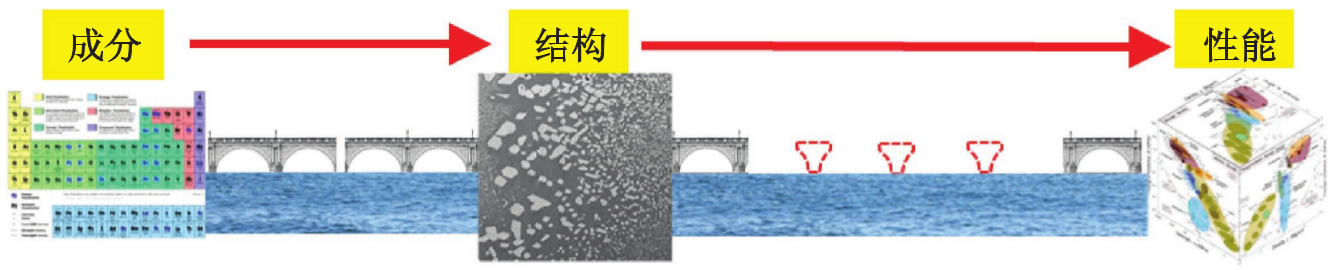
\includegraphics[height=0.80in,width=4.05in]{Figures/MGE-2.png}
%\caption{\tiny \textrm{Pseudopotential for metallic sodium, based on the empty core model and screened by the Thomas-Fermi dielectric function.}}%(与文献\cite{EPJB33-47_2003}图1对比)
\label{Multi-Scale}
\end{figure}
}

%\frame
%{
%	\frametitle{材料基因工程}
%\begin{figure}[h!]
%\vspace*{-0.18in}
%\centering
%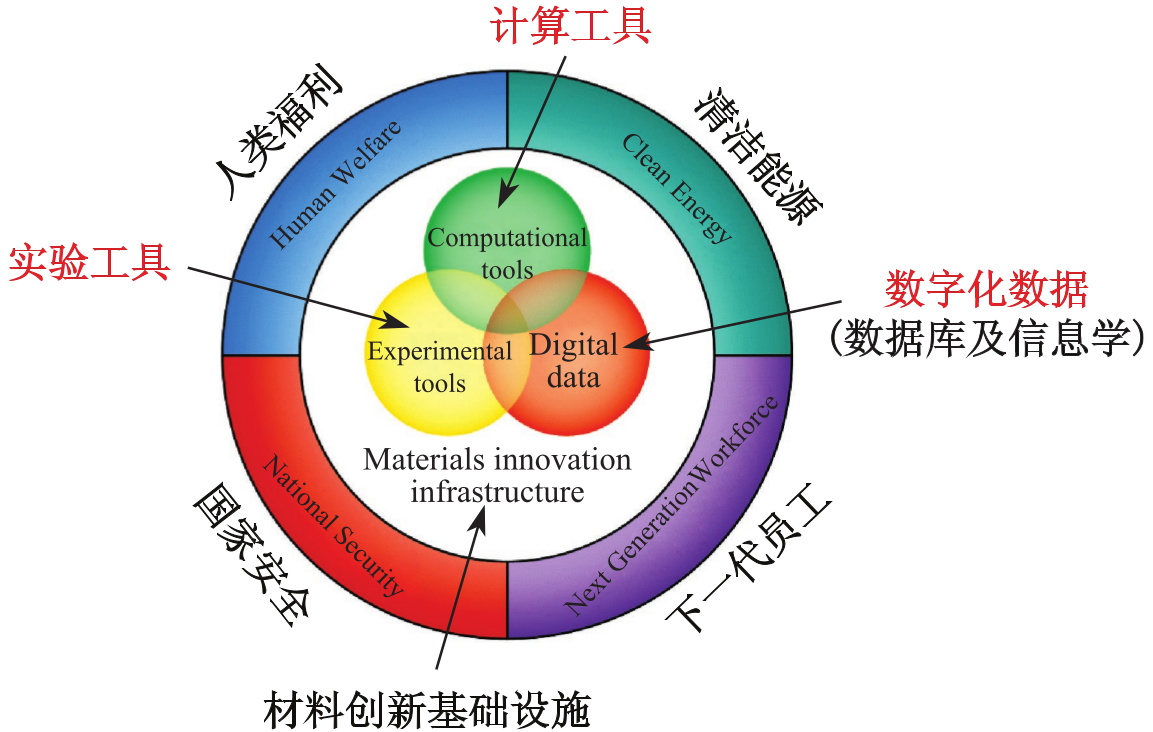
\includegraphics[height=2.55in,width=4.05in]{Figures/MGE.png}
%%\caption{\tiny \textrm{Pseudopotential for metallic sodium, based on the empty core model and screened by the Thomas-Fermi dielectric function.}}%(与文献\cite{EPJB33-47_2003}图1对比)
%%\caption{\tiny \textrm{Pseudopotential for metallic sodium, based on the empty core model and screened by the Thomas-Fermi dielectric function.}}%(与文献\cite{EPJB33-47_2003}图1对比)
%\label{MGE}
%\end{figure}
%}
\section{复杂磁性结构}
\frame
{
	\frametitle{简单磁结构~\textrm{.VS.}~复杂磁结构}
\begin{figure}[h!]
\vspace*{-0.08in}
\centering
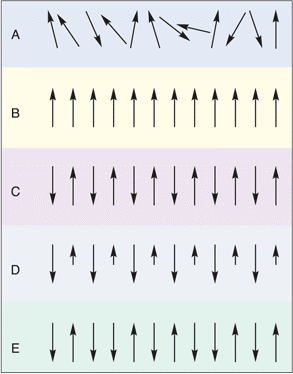
\includegraphics[height=1.05in,width=0.75in]{Figures/Magnet-simple.png}
\caption{\tiny \textrm{Simple Magnetic structure:~Ferromagnetism, Anti-Ferromagnetism, Ferrimagnetism}}%(与文献\cite{EPJB33-47_2003}图1对比)
\label{Fig:Simple-Magnet}
\end{figure}
\begin{figure}[h!]
\vspace*{-0.08in}
\centering
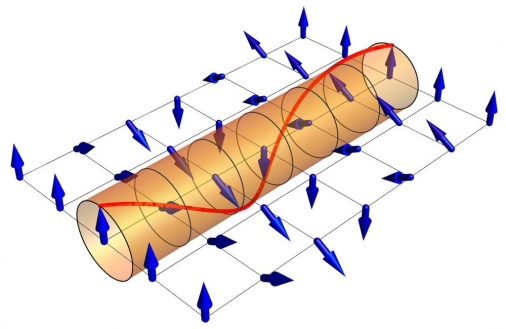
\includegraphics[height=1.05in,width=1.35in]{Figures/Magnet-complex.png}
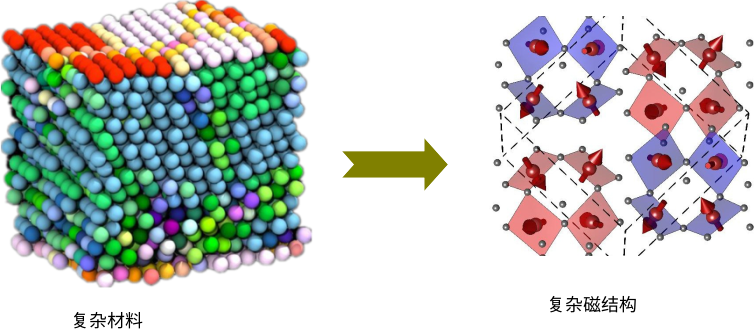
\includegraphics[height=1.05in,width=2.35in]{Figures/Magnet-complex-compound.png}
\caption{\tiny \textrm{Complex Magnetic structure:~Spiral magnet, All-in-all-out, 3k-ordered}}%(与文献\cite{EPJB33-47_2003}图1对比)
\label{Fig:Simple-Magnet}
\end{figure}
}

\frame
{
	\frametitle{复杂磁结构的两大起源}
	\begin{itemize}
		\item 强磁阻挫:~\textrm{Kagome}晶格
\begin{figure}[h!]
\vspace*{-0.08in}
\centering
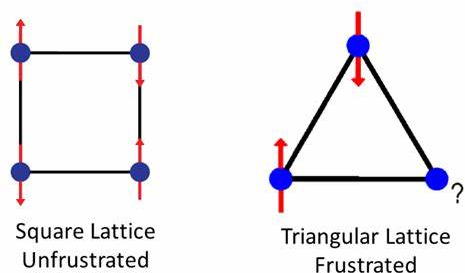
\includegraphics[height=0.8in,width=1.7in]{Figures/Magnet-Kagome-lattice.png}
\caption{\tiny \textrm{The Kagome lattice}}%(与文献\cite{EPJB33-47_2003}图1对比)
\label{Fig:Magnet-Kamoge}
\end{figure}
		\item 强自旋-轨道耦合:~稀土、锕系元素,核材料
\begin{figure}[h!]
\vspace*{-0.08in}
\centering
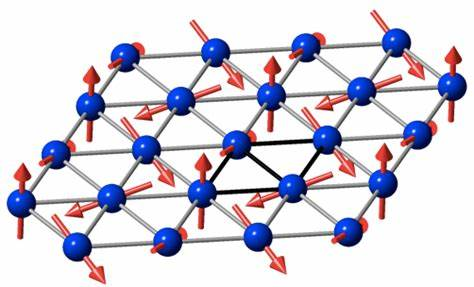
\includegraphics[height=0.75in,width=1.4in]{Figures/Magnet-Strong-SOC.png}
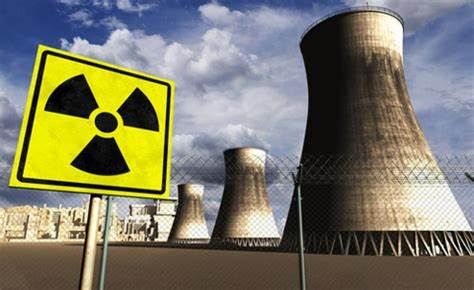
\includegraphics[height=0.75in,width=1.4in]{Figures/Nuclear-Power.png}
\caption{\tiny \textrm{Strong spin-orbit coupling and nuclear materials.}}%(与文献\cite{EPJB33-47_2003}图1对比)
\label{Fig:Magnet-SOC}
\end{figure}
	\end{itemize}
}

\section{遗传算法与结构预测}
\frame
{
	\frametitle{确定磁结构的方法和困难}
	\begin{itemize}
                \setlength{\itemsep}{5pt}
		\item \textcolor{blue}{确定磁结构的常用方法}
			\begin{enumerate}
                                \setlength{\itemsep}{3pt}
				\item 实验方法:~中子散射
				\item 理论方法:~人工猜测-计算验证方法
				\item 理论方法:~拟合磁自由度\textrm{Hamiltonian}-模拟退火
			\end{enumerate}
		\item \textcolor{blue}{复杂磁有序结构测定的困难}
			\begin{enumerate}
                                \setlength{\itemsep}{3pt}
				\item 中子散射:~某些实验材料质量欠佳、极端条件
				\item 人工猜想-计算验证方法:~效率低下,不适合复杂材料
				\item \textrm{Hamiltonian}-模拟退火:~\textrm{Hamiltonian}拟合困难,精度无法保证
			\end{enumerate}
			\textcolor{red}{本质的困难}:~海量潜在的可能结构导致常用方法失效
	\end{itemize}
}

\frame
{
	\frametitle{深度神经网络与遗传算法}
当前的深度神经网络~\textrm{(Deep Learning Neural Network)}~可以包含上百层神经元,通常有上万个参数,再加上超参数,实际的参数空间几乎是无限大的。如何从海量潜在的可能参数中做选择极具挑战性。
\begin{figure}[h!]
\vspace*{-0.08in}
\centering
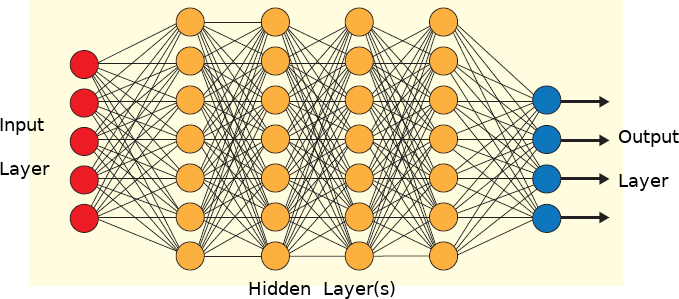
\includegraphics[height=1.75in,width=3.75in]{Figures/ANN_Algorithm.png}
\caption{\tiny \textrm{Deep Learning Neural Network.}}%(与文献\cite{EPJB33-47_2003}图1对比)
\label{Fig:Deep-Learning-NN}
\end{figure}
}

\frame
{
	\frametitle{深度神经网络与遗传算法}
	\textcolor{blue}{深度神经网络类似问题的解决方案:~遗传算法}
\begin{minipage}[b]{0.49\textwidth}
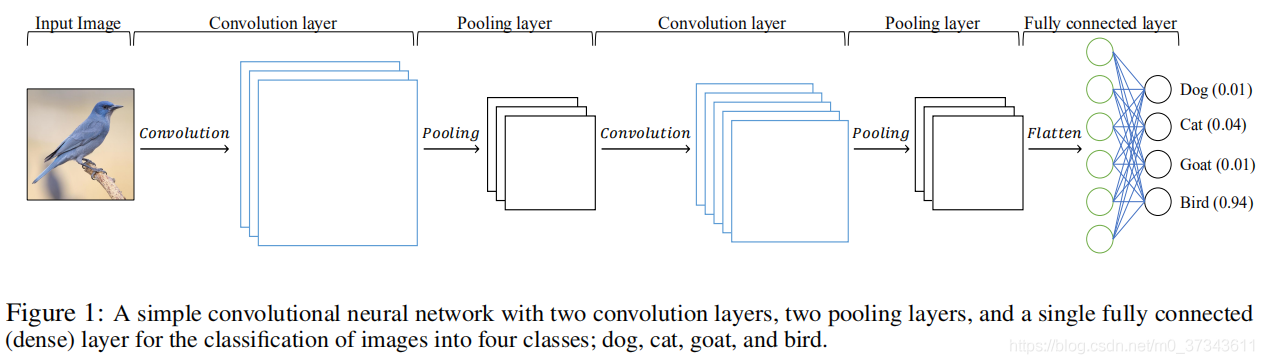
\includegraphics[height=0.4in,width=2.08in,viewport=0 110 1280 350,clip]{Figures/Genetic_Algorithm-2.png}\\
\centering{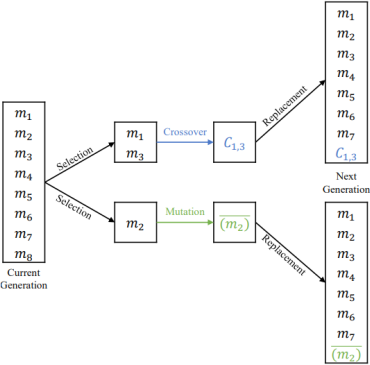
\includegraphics[height=1.0in,width=1.08in,viewport=140 50 820 650,clip]{Figures/Genetic_Algorithm-1.png}}\\
\vskip 0.02pt
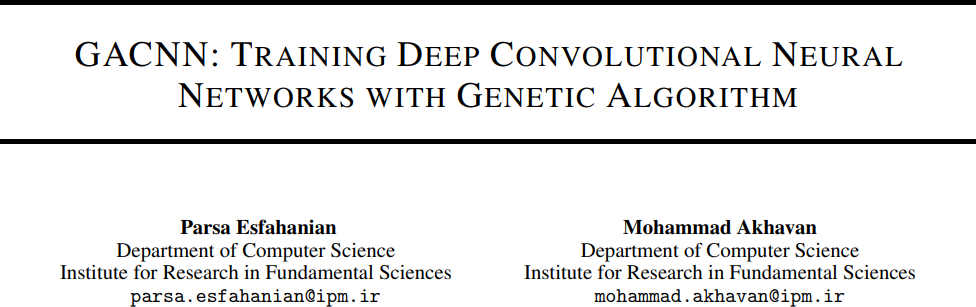
\includegraphics[height=0.7in,width=2.05in]{Figures/Genetic_Algorithm-3.png}\\
\centering{\textcolor{red}{\textrm{\tiny GACNN:~利用遗传算法训练深度卷积神经网络}}}
\end{minipage}
\hfill
\begin{minipage}[b]{0.49\textwidth}
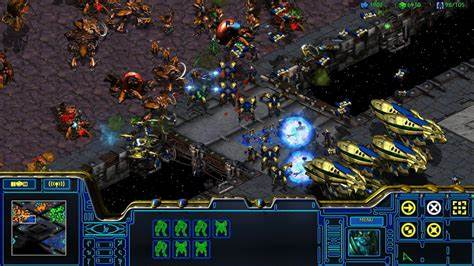
\includegraphics[height=1.2in,width=1.9in]{Figures/Genetic_Algorithm-5.png}\\
\vskip 0.5pt

\includegraphics[height=0.55in,width=1.95in]{Figures/Genetic_Algorithm-4.png}\\
\centering{\textcolor{red}{\textrm{\tiny 多智能体强化学习:~神经网络}}}
\end{minipage}
}

\frame
{
	\frametitle{晶体结构优化的复杂性}
	\begin{itemize}
		\item \textcolor{blue}{晶体结构预测与搜索中也遇到类似问题}\\
		在已知元素种类的条件下,有可能预测或搜索材料晶体的结构;~但是材料的等能面存在无数个局域极小点,因而可能的晶体结构也是无限多的\\
		这使得晶体结构的预测与搜索极其困难
\begin{figure}[h!]
\centering
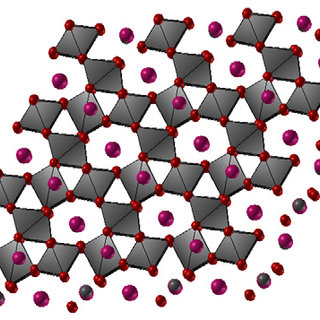
\includegraphics[height=1.3in,width=1.3in]{Figures/Struct-predict-3.png}
\hskip 1.0pt
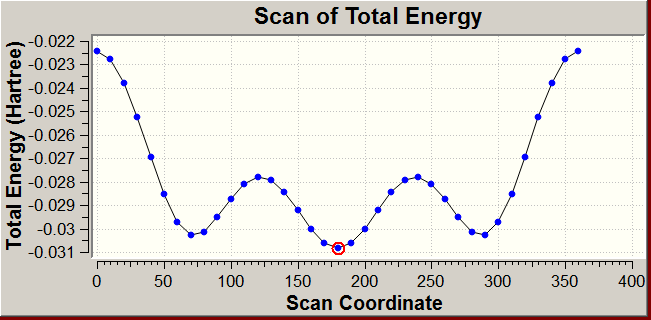
\includegraphics[height=1.2in,width=2.25in]{Figures/Total_energy_opt.png}
\caption{\tiny \textrm{The structure of Perovskite and schematic for the energy minimum searching.}}%(与文献\cite{EPJB33-47_2003}图1对比)
\label{Fig:Structure-optimized}
\end{figure}
	\end{itemize}
}

\frame
{
	\frametitle{晶体结构优化问题的解决}
	\textcolor{blue}{解决方案:~遗传算法、粒子群方法等}
\begin{figure}[h!]
\centering
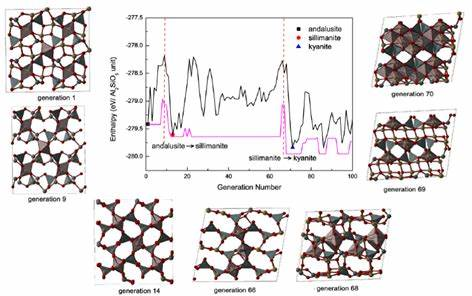
\includegraphics[height=1.0in,width=1.7in]{Figures/Struct-predict-1.png}
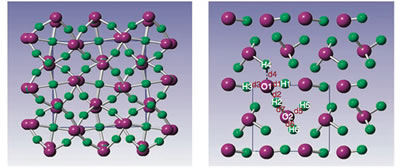
\includegraphics[height=1.0in,width=2.2in]{Figures/Struct-predict-2.png}
\vskip 8.0pt

\includegraphics[height=0.7in,width=2.2in]{Figures/Logo_USPEX.png}
\hskip 1.0pt

\includegraphics[height=1.0in,width=1.8in]{Figures/Logo_Calypso.png}
%\caption{\tiny \textrm{The structure of Perovskite and schematic for the energy minimum searching.}}%(与文献\cite{EPJB33-47_2003}图1对比)
\label{Fig:Structure-optimized-2}
\end{figure}
}

\frame
{
	\frametitle{磁结构遗传算法预测软件\textrm{MagGene}}
鉴于遗传算法在深度学习和晶体结构预测中的成功应用,这种方法在磁结构预测中也大有用武之地。\textrm{MagGene}就是整合遗传算法和常用的第一性原理计算软件预测材料磁结构新型软件。
\begin{figure}[h!]
\centering
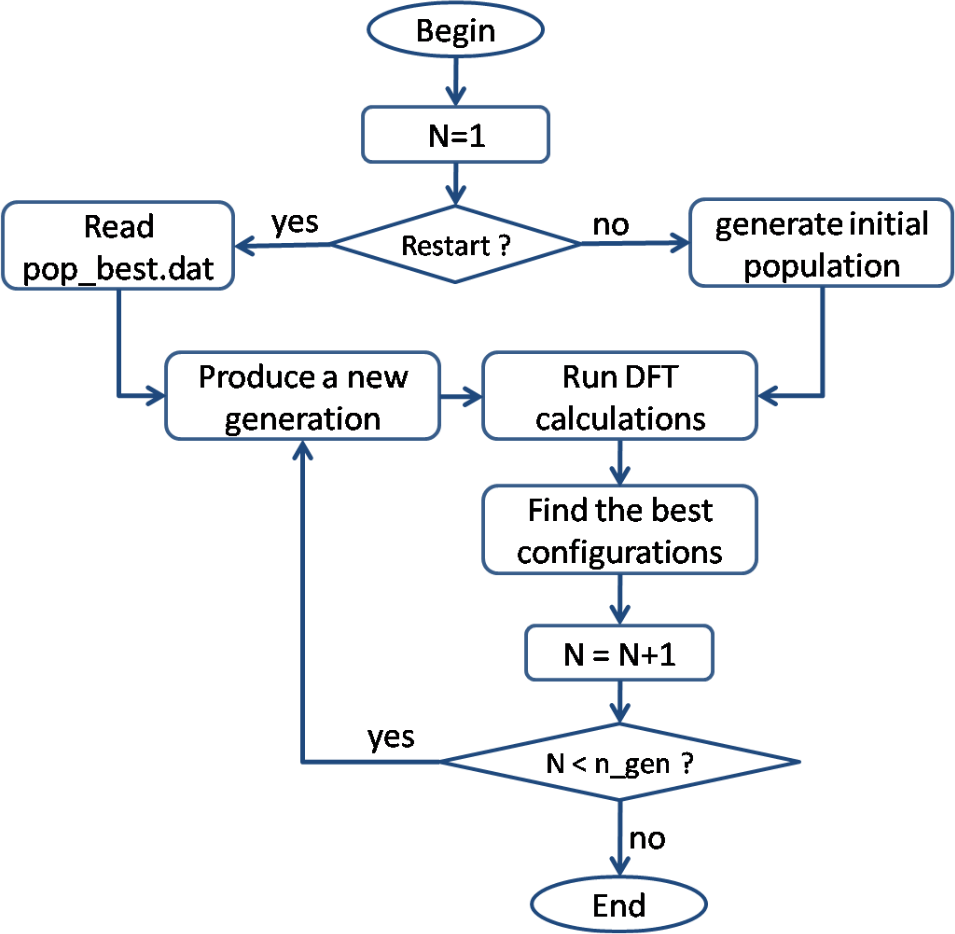
\includegraphics[height=2.2in,width=2.2in]{Figures/MagGene-Flow.png}
\caption{\tiny \textrm{The flow of MagGene.}}%(与文献\cite{EPJB33-47_2003}图1对比)
\label{Fig:MagGene-Flow}
\end{figure}
}

\frame
{
	\frametitle{\textrm{MagGene}的主要功能}
	\begin{itemize}
                \setlength{\itemsep}{15pt}
		\item \textcolor{blue}{\textrm{MagGene}的主要功能}:
			\begin{enumerate}
                                \setlength{\itemsep}{10pt}
				\item 自动产生可能的磁结构
				\item 自动生成第一性原理程序的输入文件
				\item 自动分析第一性原理程序的计算结果
				\item 筛选并优化磁结构,反复迭代,直至最终得到基态磁结构
			\end{enumerate}
		\item \textcolor{blue}{程序语言}:~\textrm{Fortran~95}
		\item \textcolor{blue}{第一原理计算程序}:~\textrm{VASP}
	\end{itemize}
}

\frame
{
	\frametitle{\textrm{MagGene}的主要文件}
	\begin{itemize}
		\item \textcolor{blue}{主输入文件:~\textrm{input.dat}}
\begin{figure}[h!]
	\vspace{-0.10in}
\centering
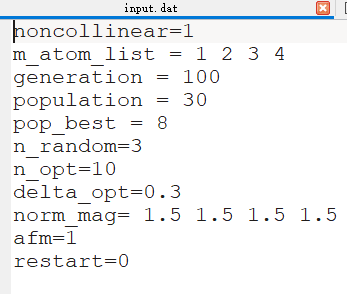
\includegraphics[height=1.0in,width=1.3in, viewport=0 20 400 290, clip]{Figures/MagGene-input.png}
%\caption{\tiny \textrm{The main input file for MagGene.}}%(与文献\cite{EPJB33-47_2003}图1对比)
\label{Fig:MagGene-input}
\end{figure}
\item \textcolor{blue}{第一性原理程序调用脚本:~\textrm{submit.sh}}
\begin{figure}[h!]
	\vspace{-0.08in}
\centering
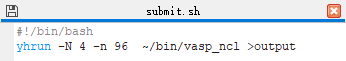
\includegraphics[height=0.3in,width=1.8in, viewport=0 0 320 60, clip]{Figures/MagGene-submit-VASP.png}
%\caption{\tiny \textrm{The script for VASP in MagGene.}}%(与文献\cite{EPJB33-47_2003}图1对比)
\label{Fig:MagGene-script-VASP}
\end{figure}
\item \textcolor{blue}{第一原理程序输入文件:}\\
	\vspace{0.08in}
	\textcolor{magenta}{\textbf{INCAR, POSCAR, KPOINTS, POTCAR}}
	\end{itemize}
}

\frame[allowframebreaks]
{
	\frametitle{\textrm{MagGene}的主要输入参数}
	\begin{itemize}
                \setlength{\itemsep}{12pt}
		\item \textcolor{purple}{\textrm{noncollinear}}:~ 0~或~1;~指定是否在非共线磁有序中搜索基态
		\item \textcolor{purple}{\textrm{restart}}:~ 0~或~1;~指定当前计算是否是续算
		\item \textcolor{purple}{\textrm{m\_atom\_list}}:~ 整数序列;~指定哪些原子带有磁性
		\item \textcolor{purple}{\textrm{generation}}:~ 整数;~指定最大遗传算法代数
		\item \textcolor{purple}{\textrm{population}}:~ 整数;~指定一代中的结构数
		\item \textcolor{purple}{\textrm{similarity\_criteria}}: 实数;~指定两个结构是否相同的判定标准
		\item \textcolor{purple}{\textrm{pop\_best}}:~ 整数;~指定每代中保留的最佳结构数
		\item \textcolor{purple}{\textrm{n\_random}}:~ 整数;~在每代中随机生成的结构数
		\item \textcolor{purple}{ \textrm{n\_mutation}}:~ 整数;~在没代中引入的变异结构数
		\item \textcolor{purple}{\textrm{delta\_mutation}}:~ 整数;~变异程度
		\item \textcolor{purple}{\textrm{norm\_mag}}:~ 实数序列;~指定每个原子的磁矩大小
		\item \textcolor{purple}{\textrm{fixm}}:~ 一个或三个实数;~限定系统总磁矩大小
		\item \textcolor{purple}{\textrm{afm}}:~ 0或1;~是否进行反铁磁结构搜索
		\item \textcolor{purple}{\textrm{dft\_coverage}}:~ 0或1;~是否抛掉密度泛函计算中未收敛的结构
	\end{itemize}
}

\section{\rm{MagGene}应用算例}

%-----------------------------------------------------------------------------------------------------------------------------------------------------------------------%
\appendix
%------------------------------------------------------------------------Reference----------------------------------------------------------------------------------------------
%\frame
%{
%\frametitle{主要参考文献}
%\begin{thebibliography}{99}
%{\small
%\bibitem{Singh_Book}\textrm{D. J. Singh. \textit{Plane Wave, PseudoPotential and the LAPW method} (Kluwer Academic, Boston,USA, 1994)}					%
%\end{thebibliography}
%  \nocite{*}																				%
%}
%}

%-----------------------------------------------------------Beamer下不建议使用bib,因为涉及分页--------------------------------------------------------------------------%
%\frame[allowframebreaks]
%{
%\frametitle{主要参考文献}
%{\tiny\textrm{
%%\phantomsection\addcontentsline{toc}{section}{Bibliography}	 %直接调用\addcontentsline命令可能导致超链指向不准确,一般需要在之前调用一次\phantomsection命令加以修正	%
%%\phantomsection\addcontentsline{toc}{section}{主要参考文献}	 %直接调用\addcontentsline命令可能导致超链指向不准确,一般需要在之前调用一次\phantomsection命令加以修正	%
%\bibliography{Ref_2020-11-28}%
%\bibliographystyle{../ref/mybib}%
%}}
%\nocite{*}%
%}
%------------------------------------------------------------------------------------------------------------------------------------------------------------------------------%

%------------------------------------------------------------------------Reference----------------------------------------------------------------------------------------------
%\begin{thebibliography}{99}
%-----------------------------------------------------------------------------------------------------------------------------------------------------------------------%
%\frame
%{
%\frametitle{主要参考文献}
%{\small
%\bibitem{Singh_Book}\textrm{D. J. Singh. \textit{Plane Wave, PseudoPotential and the LAPW method} (Kluwer Academic, Boston,USA, 1994)}					%
%  \nocite{*}																				%
%}
%}
%\end{thebibliography}

%-----------------------------------------------------------Beamer下不建议使用bib,因为涉及分页--------------------------------------------------------------------------%
%\frame[allowframebreaks]
%{
%\frametitle{主要参考文献}
%{\tiny\textrm{
%%\phantomsection\addcontentsline{toc}{section}{Bibliography}	 %直接调用\addcontentsline命令可能导致超链指向不准确,一般需要在之前调用一次\phantomsection命令加以修正	%
%%\phantomsection\addcontentsline{toc}{section}{主要参考文献}	 %直接调用\addcontentsline命令可能导致超链指向不准确,一般需要在之前调用一次\phantomsection命令加以修正	%
%\bibliography{../ref/Myref}																			%
%\bibliographystyle{../ref/mybib}																		%
%}}
%\nocite{*}																				%
%}
%------------------------------------------------------------------------------------------------------------------------------------------------------------------------------%

%-------------------------------------------------------------------------Thanks------------------------------------------------------------------------------------------------
%\section{致谢}
%\frame
%{
%\frametitle{致$\quad$谢}
%\begin{itemize}
%    \setlength{\itemsep}{20pt}
%  \item 感谢本团队高兴誉、吴泉生、宋红州等各位老师参与的讨论
%  \item 感谢莫所长、宋主任以及软件中心各位老师和同事
%  \item 感谢王崇愚先生的帮助
%\end{itemize}
%}

\logo{}									%不显示logo
\frame
{
\vskip 60 pt
%\hskip 10pt \textcolor{blue}{\Huge 感谢答辩委员会各位老师\,\textrm{!}}\\
\vskip 35 pt
\hskip 60pt \textcolor{blue}{\Huge 谢谢大家\:!}
%\vskip 15 pt
%\hskip 40pt \textcolor{blue}{\Huge \textrm{for your attention\:!}}
}

%\frame
%{
%\begin{figure}[h!]
%\centering
%\animategraphics[autoplay, loop, height=2.1in]{1}{Figures/Prof_Liu-}{06}{11}
%\label{Prof_Liu}
%\end{figure}
%}
%
%-------------------------------------------------------------------------------------------------------------------------------------------------------------------------------

\clearpage
%\end{CJK*}
\end{document}
